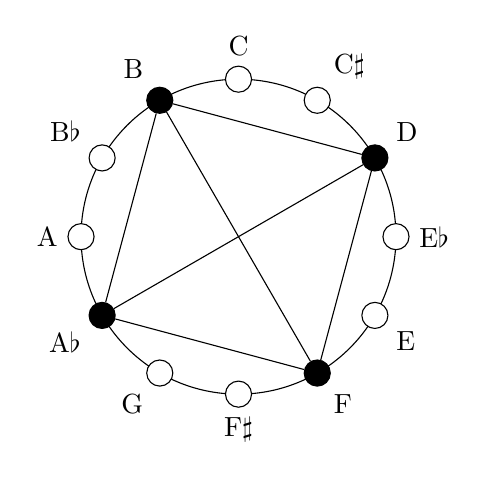
\begin{tikzpicture}[scale={2}]
\def \radius{1.0}
\node (origin) at (0,0) {};
\draw (origin) circle (\radius);
\node (n0) at +(90.0:\radius) [circle, draw, fill=white, label = 90.0:C]{};
\node (n1) at +(60.0:\radius) [circle, draw, fill=white, label = 60.0:C$\sharp$]{};
\node (n2) at +(30.0:\radius) [circle, draw, fill=black, label = 30.0:D]{};
\node (n3) at +(0.0:\radius) [circle, draw, fill=white, label = 0.0:E$\flat$]{};
\node (n4) at +(330.0:\radius) [circle, draw, fill=white, label = 330.0:E]{};
\node (n5) at +(300.0:\radius) [circle, draw, fill=black, label = 300.0:F]{};
\node (n6) at +(270.0:\radius) [circle, draw, fill=white, label = 270.0:F$\sharp$]{};
\node (n7) at +(240.0:\radius) [circle, draw, fill=white, label = 240.0:G]{};
\node (n8) at +(210.0:\radius) [circle, draw, fill=black, label = 210.0:A$\flat$]{};
\node (n9) at +(180.0:\radius) [circle, draw, fill=white, label = 180.0:A]{};
\node (n10) at +(150.0:\radius) [circle, draw, fill=white, label = 150.0:B$\flat$]{};
\node (n11) at +(120.0:\radius) [circle, draw, fill=black, label = 120.0:B]{};
\draw[solid] (n2) -- (n5);
\draw[solid] (n2) -- (n8);
\draw[solid] (n2) -- (n11);
\draw[solid] (n5) -- (n8);
\draw[solid] (n5) -- (n11);
\draw[solid] (n8) -- (n11);
\end{tikzpicture}
